%-----------------------------------------------------------------------------
%
%          PHYSICS  M.S.     THESIS
%          JUSTIN A. VASEL
%
%          This began as the template offered by the University of Minnesota, 
%          but I've made a few changes here and there...  
%
%          -->  halo.tex
%
%-----------------------------------------------------------------------------


\chapter{Helium and Lead Observatory}
	\label{halo_chapter}

	\begin{quoting}
		\noindent \large ``Astronomically Patient" \normalsize

		--- The HALO Collaboration
	\end{quoting}

	\chapterIntro{B}{uried 6,800 feet below ground,} SNOLAB is the deepest laboratory in the world. SNOLAB is located near Sudbury, Ontario, Canada in the Vale Creighton Mine. Originally, the laboratory consisted of just one experiment, the Sudbury Neutrino Observatory (SNO). Due to the success of SNO in shedding light on the solar neutrino problem, the laboratory expanded and now is home to a handful of neutrino and dark matter experiments. The Helium and Lead Observatory (HALO) is one of the experiments that calls SNOLAB its home. 

	The HALO experiment is currently in the final stages of development. When it is complete, HALO will continuously search for the distinct neutrino signal produced during a galactic supernova as a member of SNEWS. HALO is unique in that it is the only neutrino experiment whose primary objective is to detect supernova neutrinos.

	\begin{figure}[H]
		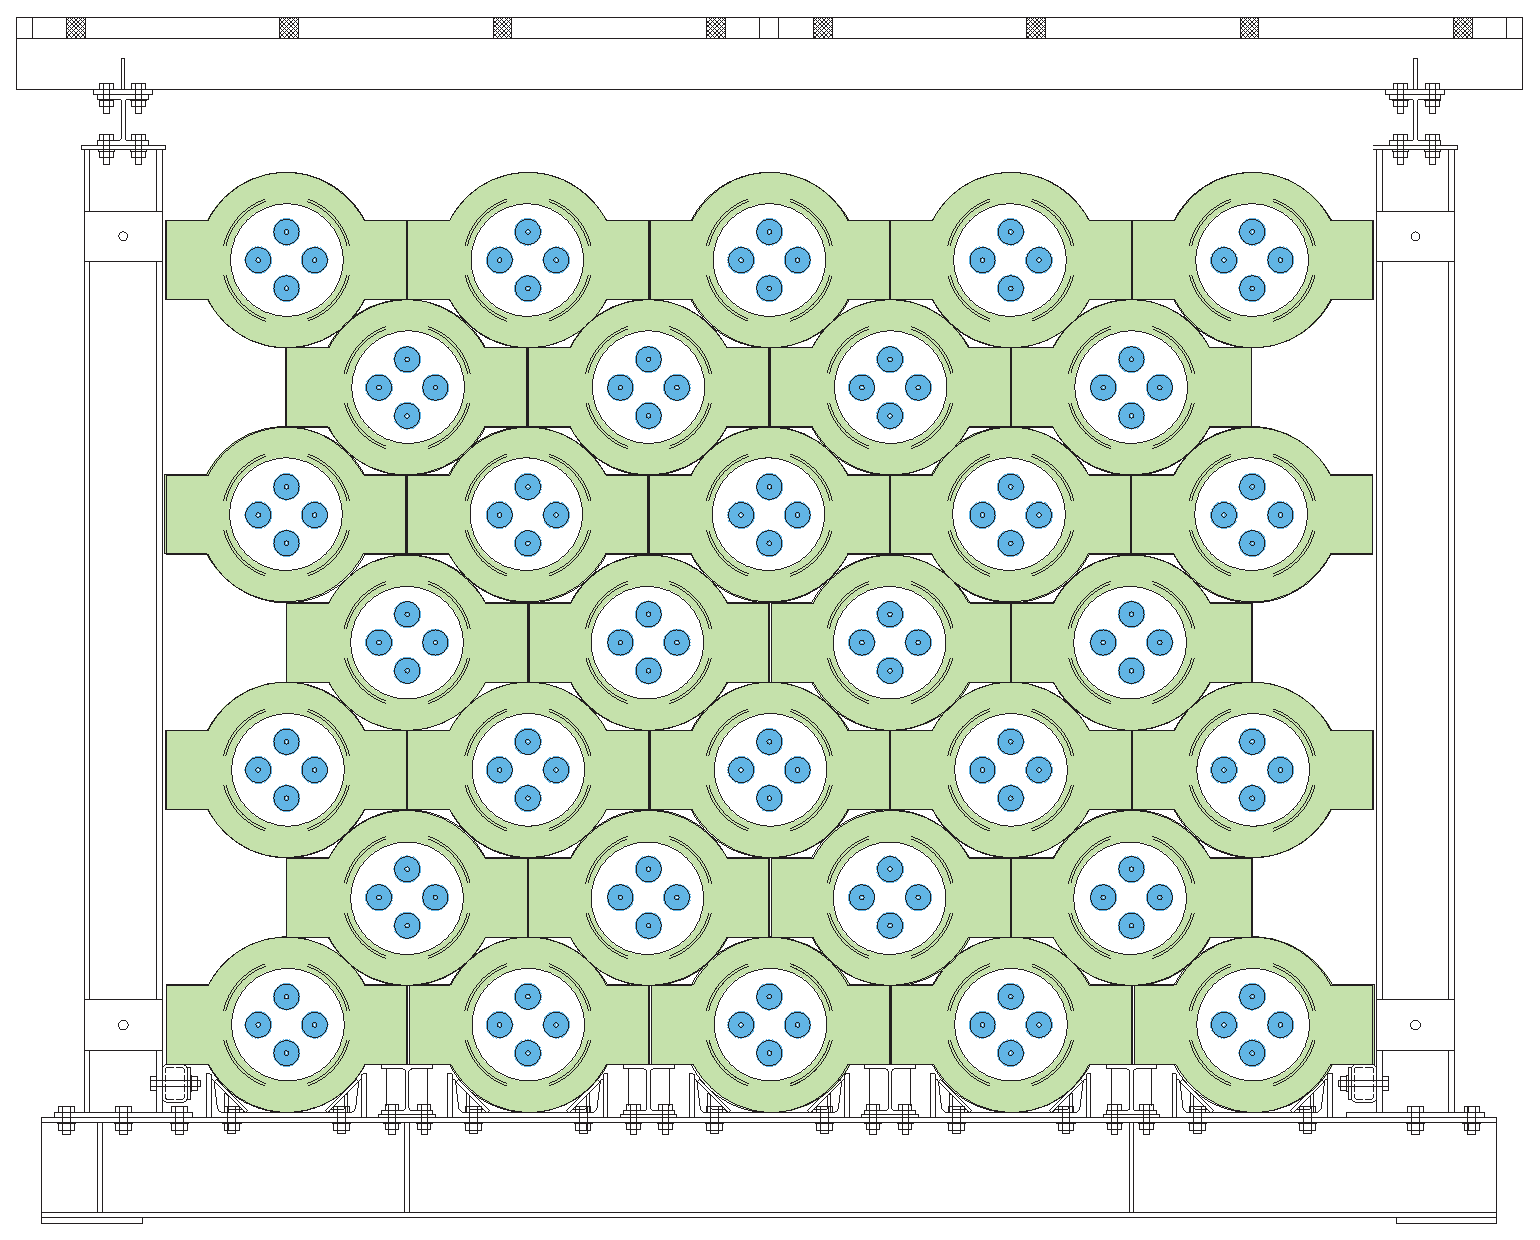
\includegraphics[width=\textwidth]{halo_diagram}
		\caption[The HALO Detector]{\bf Schematic of the HALO detector design. \rm The lead bores are shaded green. The \he proportional counters are shaded blue.}
		\label{fig:halo}
	\end{figure}

	The HALO detector consists of \ \SI[mode=text]{76}{tons} of lead and 128 \he neutron detectors. The lead serves as the interaction medium and is sectioned in blocks. Each block of lead has a bore through the middle of it within which sit four \he neutron detectors \nolinebreak (\FIG \ref{fig:halo}).

	Because galactic supernovae only occur two or three times each century\cite{sn_rates}, HALO is designed with longevity in mind. Once completed, the experiment will be highly automated and relatively inexpensive to maintain, allowing it to remain in operation for decades. 



	%% SECTION : LEAD AS AN INTERACTION MEDIUM
	\section{Lead as a Interaction Medium}

	HALO is the only neutrino experiment that uses lead as an interaction medium. Lead was chosen because it was economical, available, and efficiently delivers neutrons to the \he neutron counters in which detection actually occurs. Lead has a relatively high neutrino interaction cross section which results in the production of neutrons\cite{Engel2003}. These interactions are described as neutral current (NC), which are moderated by the $\HepParticle{\PZzero}{}{}$ boson (\EQ \ref{eq:nc}), or charged current (CC), which are moderated by the $\HepParticle{\PWpm}{}{}$ bosons (\EQS \nolinebreak \ref{eq:nue_cc}, \nolinebreak \ref{eq:nue_bar_cc})\footnote{A fourth type of neutrino interaction is elastic scattering (ES) in which a neutrino scatters off of an electron (\HepProcess{\HepParticle{\Pnue}{}{} + \HepParticle{\Pelectron}{}{} \to \HepParticle{\Pnue}{}{} + \HepParticle{\Pelectron}{}{}}). Some neutrino detectors are sensitive to this type of interaction, but HALO is not because it cannot detect electrons.}.

		\begin{align}
			\quad \textbf{Neutral Current} \qquad &\HepProcess{\HepParticle{\Pneutrino}{}{} + \text{Pb} \to \HepParticle{\Pneutrino}{}{*} + \text{Pb}^*} \label{eq:nc} \\
			\quad \textbf{$\HepParticle{\Pnue}{}{}$ Charged Current} \qquad &\HepProcess{\HepParticle{\Pnue}{}{} + \text{Pb} \to \HepParticle{\Pelectron}{}{} + \text{Bi}^*} \label{eq:nue_cc} \\
			\quad \textbf{$\HepParticle{\APnue}{}{}$ Charged Current} \qquad &\HepProcess{\HepParticle{\Pnue}{}{} + \HepParticle{\Pproton}{}{} \to \HepParticle{\Ppositron}{}{} + \HepParticle{\Pneutron}{}{}} \label{eq:nue_bar_cc}
		\end{align}

		\begin{figure}[H]
			
\includegraphics[width=\textwidth]{total}
			\caption[Neutrino Detector Sensitivities]{\bf Neutrino detector sensitivities. \rm Since HALO is the first experiment to lead as an interaction medium, it will offer unique insight into the $\HepParticle{\Pnue}{}{}$ charged current channel.}
			\label{fig:sensitivities}
		\end{figure}

	In NC interactions, a neutrino of any flavor strikes a lead nucleus and excites it. When the nucleus de-excites, zero, one, or two neutrons are produced ($\HepProcess{\text{Pb}^* \to \text{Pb} + \HepParticle{\Pphoton}{}{} + \text{neutrons}}$). In $\HepParticle{\Pnue}{}{}$ CC interactions, an electron neutrino interacts with a neutron in the lead nucleus, producing an electron and bismuth in an excited state. Again, the nucleus de-excites and produces zero, one, or two neutrons ($\HepProcess{\text{Bi}^* \to \text{Bi} + \HepParticle{\Pphoton}{}{} + \text{neutrons}}$).

	The third possible interaction, $\HepParticle{\APnue}{}{}$ CC, is highly suppressed due to ``pauli blocking.'' The excess of neutrons in lead makes it less likely that neutron will be produced because many of the low-energy states are already filled, and neutrons are fermionic particles that are subject to the Pauli exclusion principle. 

	\begin{wrapfigure}{l}{0.3\textwidth}
		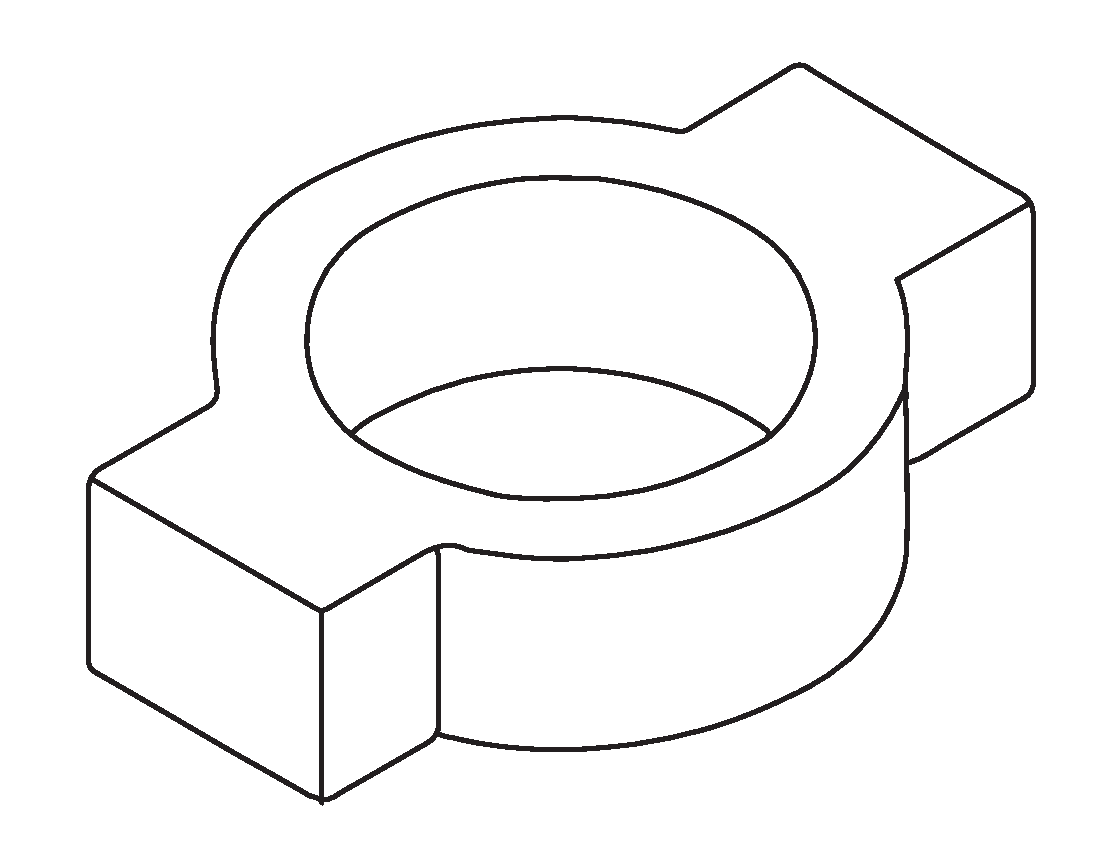
\includegraphics[width=0.3\textwidth]{lead}
		\caption[Schematic of Lead Blocks]{\bf Schematic of lead blocks. \rm}
		\label{fig:lead}
		\vspace{-0.1in}
	\end{wrapfigure}
	The lead blocks were originally used in the Deep River cosmic ray experiment. The lead is stacked in alternating rows of four and five (\FIG \ref{fig:halo}) and each row runs 3 meters deep. This geometry was chosen to maximize the number of lead blocks used while being confined to the relatively small space that HALO is given in SNOLAB. HALO makes use of 76 tons of lead; 864 blocks in total.

	The lead blocks were painted to minimize health risks associated with exposure to lead and to minimize contamination of the SNOLAB environment. The type of paint used was meticulously chosen based on several factors, including its resistance to peel or rust, its neutron-capture cross section, and its containment of radioactive isotopes that could increase background noise in the detector\cite{Shantz2010}.



	%% SECTION : 3HE PROPORTIONAL COUNTERS
	\section{\he Proportional Counters}

	The neutrons produced from nuclear de-excitation of either lead or bismuth pass into one of the 128 proportional detectors (\FIG \ref{fig:ncd}) which are filled with a gaseous mixture of \he and CF$_4$ (85/15 by volume) at a pressure of \SI[mode=text]{2.5}{atm}. The neutrons are captured on \he shortly after entering the tube by the following reaction:
	\begin{equation}
		\HepProcess{^3\text{He} + \HepParticle{\Pneutron}{}{} \to \HepParticle{\Pproton}{}{} + {}^3\text{H} + \ekeV{764}}
	\end{equation}
	Of the \ekeV{764} released from the reaction, \ekeV{573} is the kinetic energy of the proton and \ekeV{191} is the kinetic energy of the triton. The production of these charged particles ionizes the nearby gas, producing ion pairs that are accelerated in opposite directions by a coaxial anode and cathode. The electric field near the anode is strong enough to allow secondary ionization of the surrounding gas by the accelerating electrons. This produces a cascade of ionization that is ultimately collected on the anode. The amount of charge collected at the anode is proportional to the original number of ion pairs. 

	\begin{figure}[H]
		\includegraphics[width=\textwidth]{ncd}
		\caption[Technical Diagram of \he Proportional Counter]{\bf Technical diagram of \he proportional counter. \rm The counters were originally used in Phase III of the SNO experiment, but have been refitted with new endcaps for use in HALO.}
		\label{fig:ncd}
	\end{figure}

	The spectrum of neutron energies does not have a single sharp peak at \ekeV{764}, however. Instead, the spectrum has two distinct shoulders to the left of the peak (\FIG \nolinebreak \ref{fig:neutron_spectrum}). These shoulders are artifacts of the ``wall effect.'' The wall effect occurs when neutron capture happens very close to the detector wall. When the proton and triton are created, one of them may collide with the wall of the detector or be absorbed by it entirely, reducing the total kinetic energy detected by the counter.

	\begin{figure}[H]
		\centering
		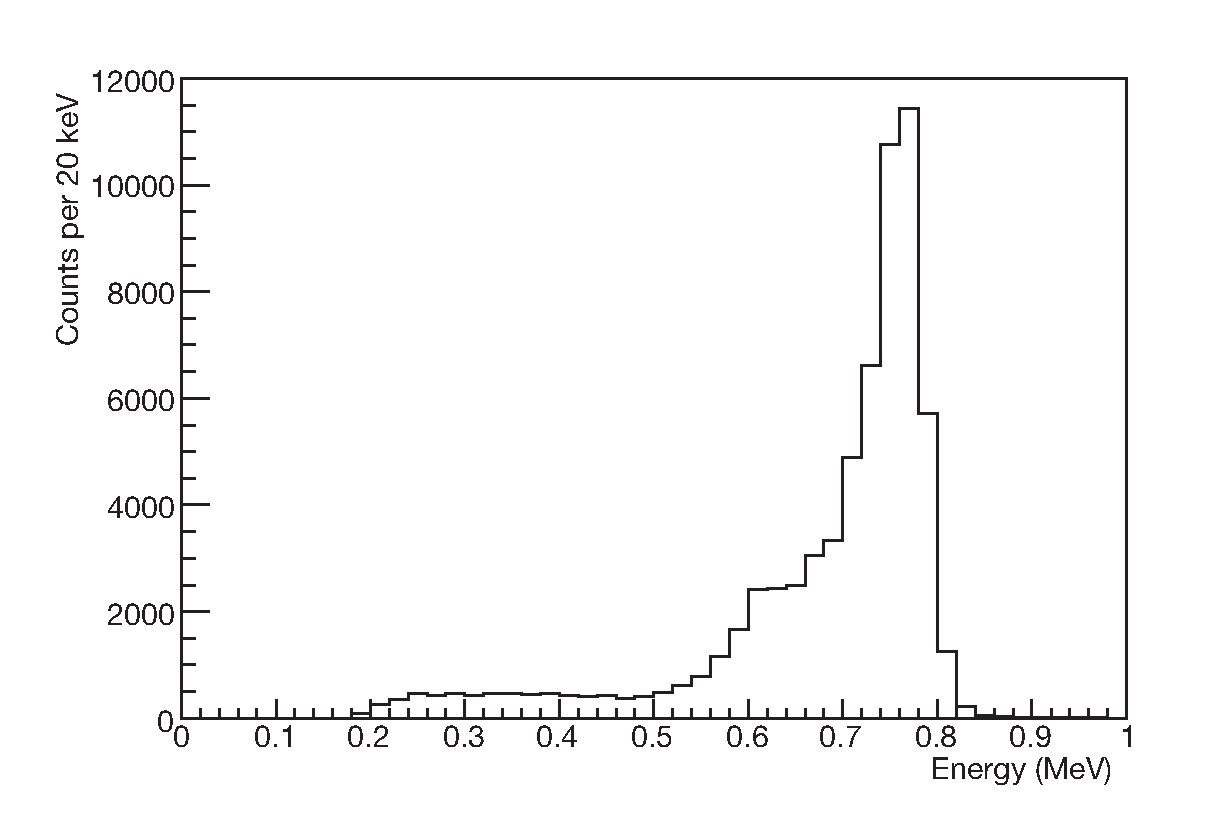
\includegraphics[width=0.9\textwidth]{neutron_spectrum}
		\caption[Example Neutron-Capture Spectrum]{\bf \he neutron-capture spectrum from $^{24}$Na calibration\rm \cite{Search2011}. The neutron peak is clearly located at \ekeV{764}, but there also exist shoulders that terminate at \ekeV{573} and \ekeV{191} due to some of the triton's or proton's energy (respectively) being lost due to collisions with the walls of the counter.}
		\label{fig:neutron_spectrum}
	\end{figure}

	Of course, the neutron spectrum is the end result of analyzing the current signals generated by the cascading electrons near the anode, which will be discussed in greater detail in \SEC \ref{sec:electronics}. The proton-triton pair move away from each other in some orientation relative to the anode at the center of the tube. The particular orientation influences the shape of the current pulse that is collected at the anode. If, when created, the proton is moving toward the anode, then the triton is moving away from the anode and the current pulse from the proton will arrive before that of the triton. If the proton and triton are produced in such a way that they both move parallel to the anode wire, then their current pulses will arrive at the anode simultaneously. 

	\begin{figure}[H]
		\centering
		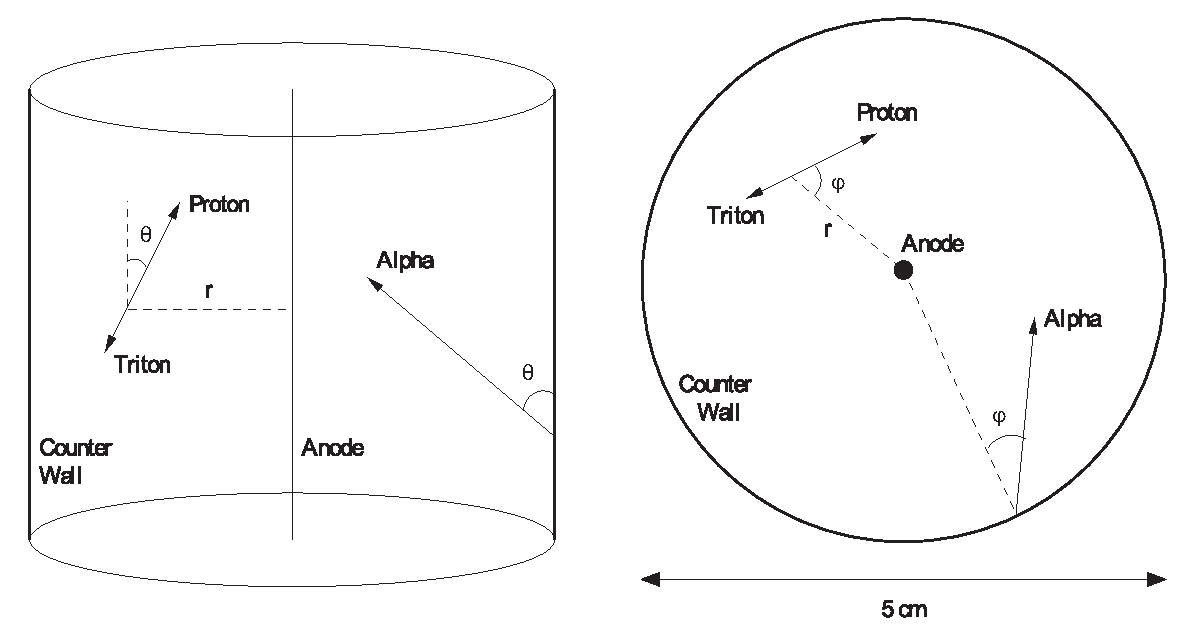
\includegraphics[width=0.9\textwidth]{capture}
		\caption[\he Neutron Capture Schematic]{\bf \he Neutron capture schematic\rm \cite{Search2011}. The proton-triton pair are produced and move in opposite directions. The proton and triton peaks may be separated in time by an amount determined by their orientation in the counter.}
		\label{fig:capture}
	\end{figure}

	%% SECTION : NEUTRON BACKGROUNDS AND NOISE
	\section{Neutron Backgrounds and Noise}
	SNOLAB is better than any other laboratory when it comes to sheilding. The \SI[mode=text]{6800}{feet} of rock that sit above it is the equivalent of \SI{6000}{\meter} of water. That notwithstanding, there is still background flux of both fast and thermal neutrons produced by radioactive decays and cosmic ray muon interactions within the surround rock. The flux of thermal and fast neutrons in SNOLAB has been measured to be \SI[mode=text]{4100}{neutrons.m^{-2}.day^{-1}} and \SI[mode=text]{4000}{neutrons.m^{-2}.day^{-1}} respectively\cite{handbook}. 

	To ensure that HALO will maintain the false-alarm rate required for participation in SNEWS (see \SEC \ref{sec:snews_positive}), shielding must be placed around the detector to block as much of the neutron background as possible. 

	\plan{MISSING CHUNK HERE ABOUT SHEILDING} 
 
	The proportional counters are very effective as long as ionization is induced by neutron capture events only. Collisions within\he gas can excite molecules without ionizing them, leading to the emission of a photon when the molecule de-excites. The photons can then go on to cause ionization elsewhere in the detector. This is the reason for the \he/CF$_4$ mixture. The CF$_4$ provides stopping power for ionizing particles, substantially reducing the effect.

	The outer shell of the\he counter is composed of ultra-pure nickel. The walls are only \SI{380}{\micron} thick and were produced in a uniform way through the process of chemical vapor deposition. Despite the purity of the detector material, there are trace amounts of radioactive nuclei that contribute to noise in the signal. The most common byproduct of radioactive decays are $\alpha$ particles. The $\alpha$ particles can interact with other elements resulting in the production of a neutron. Fortunately, $\alpha$ particles have charge and are very heavy and so they have a very short range. This prevents them in many cases from arriving at the detector wall with sufficient energy to initiate radioactive decay. 

	The few neutrons that are produced by interactions with $\alpha$ particles have energies that are a couple tens of \eMeV{}, making them indistinguishable from neutrons produced by supernova neutrino interactions. A study of these $\alpha$ backgrounds found that the rate of neutron-producing $\alpha$ particles was $21.9^{+1.1}_{-1.0}$ per day and is considered negligable\cite{Shantz2010}. 

	Gamma rays are another source of noise and are produced through nuclear decays of uranium and thorium found in the paint that coats the lead blocks. Uranium and thorium decay via $\alpha$ or $\beta$ emission, but the decay of daughter nuclei can produce gammas. These photons can interact with electrons via Compton scattering and cause the electrons to move. Multiple scattering effects may imbue the electrons with enough energy to survive being cut by detector electronics, resulting in the false count of a neutron. Simulations\cite{Shantz2010} and HALO data show that the energy of these gamma-induced counts tends to be less than a few \eMeV{}, making them easily distinguishable from the neutrino-induced neutron signal.

 	%% SECTION : DETECTOR ELECTRONICS AND DATA FLOW
	\section{Detector Electronics and Data Acquisition}
	\label{sec:electronics}
		\filler


%-----------------------------------------------------------------------------
%-----------------------------------------------------------------------------